\documentclass[thesis,fonts=libertine]{cluu}

\usepackage[style=cluu]{biblatex}
\usepackage{amsmath}
\usepackage{tikz}
\usepackage{graphicx}

\graphicspath{ {figures/} }
\addbibresource{thesis.bib}

\usepackage{pythonhighlight}    % for \inputpython at the end

\begin{document}
\author{Shifei Chen}
\supervisors{Ali Basirat, Uppsala University}
\title{Palindromes}
\subtitle{Never odd or even}

\maketitle

\begin{abstract}
  The concept of \emph{palindromes} is introduced, and some method for
  finding palindromes is developed.
\end{abstract}

\tableofcontents

\addchap{Preface}

This thesis was finished under the supervision from Ali Basirat. I would like 
to thank him for his continuous help and inspriration.

I would like to thank Mr. Anders Wall and everyone in the Anders Wall Scholarship Foundation for sponsoring my Master study. I would also like to thank everyone in the Master Programme in Language Technology, including all of my classmates and the teachers. I have learned a lot from you during this 2-years journey.

Last but not least, I would like to say thank you to my parents for their unconditional love and support. Also to my girlfriend, who has always been together with me during this unusual time.

% by using \addchap instead of \chapter this preface isn't numbered.

\chapter{Introduction}

Palindromes are fun. I've tried to find some.
In Chapter \ref{chap:prev} previous work is reviewed, and
Chapter \ref{chap:results} is about my results.

\chapter{Previous work}
\label{chap:prev}

\section{Word Embeddings}
\subsection{Representing Words in Vectors}

In Natural Language Processing, people need to convert the natural representation of words into form that are more effieicent for computer to process. The idea started with statistical language modelling \parencite{bengio2003neural}. In 2013, \cite{Mikolov:2013aa} introudced Word2Vec, which encapsules words and their latent information into vectors. Besides the benefit that it simplifies representation and storage of words for computers, it also enables the possibilities to calcualte word and their semantic meanings just as vectors.

Take an example vocabulary $V=\{\text{king}, \text{queen}, \text{man}, \text{woman}\}$, if we convert these words into vectors such as 

\begin{align*}
  \vec{k} &= \text{vec}(\text{king})\\
  \vec{q} &= \text{vec}(\text{queen})\\
  \vec{m} &= \text{vec}(\text{man})\\
  \vec{w} &= \text{vec}(\text{woman})
\end{align*}

We could have an equation of 

\begin{equation}
  \label{equa:semantic_vectors}
  \vec{q}=\vec{k}-\vec{m}+\vec{w}
\end{equation}

It is meaningful from both the mathmatical prospective and the linguistic prospective. The latter can be illustrated by Figure \ref{fig:semantic_vectors} in a vector space that contains these four vectors. In addition, the two cosine similarity values of vectors $\vec{k}$ and $\vec{q}$, and of $\vec{m}$ and $\vec{w}$ should also be close, as the angles between each two vectors are about the same.

\begin{figure}
  \centering
  \tikzset{every picture/.style={line width=0.75pt}} %set default line width to 0.75pt
  \begin{tikzpicture}[x=0.75pt,y=0.75pt,yscale=-1,xscale=1]
    %uncomment if require: \path (0,256); %set diagram left start at 0, and has height of 256

    %Shape: Axis 2D [id:dp40983147480798976]
    \draw  (49,221.35) -- (260.5,221.35)(70.15,31) -- (70.15,242.5) (253.5,216.35) -- (260.5,221.35) -- (253.5,226.35) (65.15,38) -- (70.15,31) -- (75.15,38)  ;
    %Straight Lines [id:da3468248594605029]
    \draw [color={rgb, 255:red, 74; green, 144; blue, 226 }  ,draw opacity=1 ]   (70.15,221.35) -- (91.04,133.95) ;
    \draw [shift={(91.5,132)}, rotate = 463.44] [color={rgb, 255:red, 74; green, 144; blue, 226 }  ,draw opacity=1 ][line width=0.75]    (10.93,-3.29) .. controls (6.95,-1.4) and (3.31,-0.3) .. (0,0) .. controls (3.31,0.3) and (6.95,1.4) .. (10.93,3.29)   ;
    %Straight Lines [id:da060011766798584776]
    \draw [color={rgb, 255:red, 80; green, 227; blue, 194 }  ,draw opacity=1 ][fill={rgb, 255:red, 182; green, 34; blue, 34 }  ,fill opacity=1 ]   (70.15,221.35) -- (98.61,163.79) ;
    \draw [shift={(99.5,162)}, rotate = 476.31] [color={rgb, 255:red, 80; green, 227; blue, 194 }  ,draw opacity=1 ][line width=0.75]    (10.93,-3.29) .. controls (6.95,-1.4) and (3.31,-0.3) .. (0,0) .. controls (3.31,0.3) and (6.95,1.4) .. (10.93,3.29)   ;
    %Straight Lines [id:da268618270283273]
    \draw [color={rgb, 255:red, 208; green, 2; blue, 27 }  ,draw opacity=1 ]   (70.15,221.35) -- (127.85,182.12) ;
    \draw [shift={(129.5,181)}, rotate = 505.79] [color={rgb, 255:red, 208; green, 2; blue, 27 }  ,draw opacity=1 ][line width=0.75]    (10.93,-3.29) .. controls (6.95,-1.4) and (3.31,-0.3) .. (0,0) .. controls (3.31,0.3) and (6.95,1.4) .. (10.93,3.29)   ;
    %Straight Lines [id:da46956564149919644]
    \draw [color={rgb, 255:red, 245; green, 166; blue, 35 }  ,draw opacity=1 ]   (70.15,221.35) -- (131.69,192.84) ;
    \draw [shift={(133.5,192)}, rotate = 515.14] [color={rgb, 255:red, 245; green, 166; blue, 35 }  ,draw opacity=1 ][line width=0.75]    (10.93,-3.29) .. controls (6.95,-1.4) and (3.31,-0.3) .. (0,0) .. controls (3.31,0.3) and (6.95,1.4) .. (10.93,3.29)   ;

    % Text Node
    \draw (83,108) node [anchor=north west][inner sep=0.75pt]   [align=left] {$\vec{k}$};
    % Text Node
    \draw (101,142) node [anchor=north west][inner sep=0.75pt]   [align=left] {$\vec{q}$};
    % Text Node
    \draw (132,166) node [anchor=north west][inner sep=0.75pt]   [align=left] {$\vec{m}$};
    % Text Node
    \draw (138,183) node [anchor=north west][inner sep=0.75pt]   [align=left] {$\vec{w}$};
  \end{tikzpicture}
  \caption{Illustraion of a vector space where Equation \ref{equa:semantic_vectors} exists.}
  \label{fig:semantic_vectors}
\end{figure}

To turn words into vectors, one could use simple one-hot encoding. Like in the example above we could make $\vec{k}=[1, 0, 0, 0]$. But these one-hot vectors can merely capture any latent semantic meanings between different words. Recent vectorized word representations, or word embeddings, were learned through neural networks, such as Word2Vec which learns word embeddings through a Skip-gram model or a Continuous Bag of Words model \parencite{Mikolov:2013ab}.

\subsubsection{The Skip-gram model}

When given a target word $w$, the model can produce vector representations that are good at predicting the words surrounding $w$ within the context size of $C$. The probability of a context word $w_k$ given a target word $w$ is:

\begin{equation}
  P(w_k|w)=\frac{\exp({v_{w_k}^\prime}^\intercal v_w)}{\sum_{i=1}^{|V|}\exp({v^\prime_i}^\intercal v_w)}
\end{equation}

Here $|V|$ means the size of the whole vocabluary from the corpus, $v^\prime$ and $v$ stand for the vector representation of the input and the output vector representation of a word \parencite{Mikolov:2013aa}. The input representation $v^\prime$ could be initialized by one-hot representations.

\subsubsection{The Continuous Bag of Words model (CBOW)}

The other model, CBOW, works just as the other side the coin. It predicts the target word $w$ based on a bunch of context words $w_{-C}, w_{-C+1} ..., w_{C-1}, w_C$ within the window size $C$, as the formula below:

\begin{equation}
  P(w|w_{-C}, w_{-C+1} ..., w_{C-1}, w_C)=\frac{\exp({v^\prime_w}^\intercal \bar{v}_{w_k})}{\sum^{|V|}_{i=1}\exp({v^\prime_{w_i}}^\intercal \bar{v}_{w_k})}
\end{equation}

Here $\bar{v}_{w_k}$ means the sum of the context word $w_k$'s vectorized representation, while $v^\prime_w$ means the input vector representationq of word $w$ as in the Skip-gram model. 

The difference between these two models is that the CBOW model predicts the target word from multiple given context words, while the Skip-gram model predicts the context words from one given center word. Hence the skip-gram model is better at predicting rare words because all of the words are treated equally in the \textit{word AND context} relationship. But in the CBOW model, common words have advantages over rare words as they will have higher probability in a given context. The Skip-gram model is arguably the most popular method to learn word embeddings as it is both fast and robust \parencite{levy-etal-2015-improving}.

\subsection{Cross-Lingual Word Embeddings}

Vectorized word representations tends to cluster words that are semantically similar to each other. It then become very attractive to see whether we could fit two or more langauges into the same vector space. This is so called multilingual word embeddings.

In such case, it is then vital to align words in two different vector spaces. As show in Fig. \ref{fig:vec_space_align}, which illustrated the alignment method from \cite{Mikolov:2013ac}. The two vector spaces were aligned by learing a rotation matrix $W$ as in process \textbf{(B)}. $W$ is then further refined in process \textbf{(C)}, where frequent words were selected as anchor points and the distance between each corrospondent anchor points were the target funciton to minimize. The final result is shown in process \textbf{(D)}.

\begin{figure}
  \label{fig:vec_space_align}
  \centering
  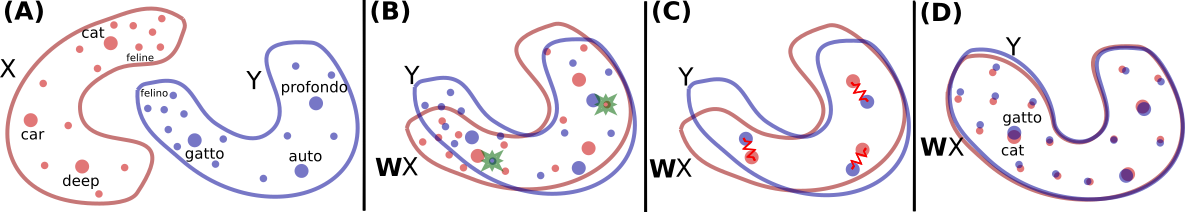
\includegraphics[width=0.8\textwidth]{vector_spaces_alignment.png}
  \caption{Aligning bilingual vector spaces. \parencite{Conneau:2017aa}}
\end{figure}

The initial alignment data to for adversarial learning the rotation matrix $W$ could come from a bilingual dictionary \parencite{Mikolov:2013ac}. There are other kinds of alignment by using aligned data from sentence level, or even document level. By using word-level information, we can start with a pivot lanugage (usually English) and map each other monolingual word embeddings by looking up translation dictionaries. This could also be done starting with bilingual vector spaces, where we choose a bilingual word embedding that shares a language (typically English) with other bilingual embeddings, and choose other bilingual word embeddings by aligning their shared language subspace. Sentence-level parallel data are similar data as the corpus in Machine Translation (MT), which contains sentence-aligned texts \parencite{Hermann:2013aa}. Document-level information are more common in the form of topic-aligned or class-aligned, such as Wikipedia data \parencite{vulic-moens-2013-study}.

The alignment process of multilingual word embeddings are roughly the same as bilingual word embeddings, using parallel data from either word-level, sentence-level or document-level. \parencite{Ruder:2019aa}.

\subsection{fastText}

\subsection{Multilingual Neural Machine Translation Systems (Using Aligned Word Embeddings)}

One of the potential application of multilingual word embeddings is machine translation. In cases where people need to translate from or into a low-resource langauge, they usually find it difficult to locate enough parallel data that consists of such kind of less common language. If we could build up a vector space with word embeddings from different languages that are aligned, we could leverage the similarity of word embeddings to compensate the lack of parallel data \parencite{zou-etal-2013-bilingual}. We could find words that are never seen in the training data buy looking for their neighbours in the vector space. There are case where successfully trained a machine translation system using very little or none parallel data \parencite{Conneau:2017aa}.

\section{Language Embeddings}

\section{Machine Translation}

\chapter{Methodalogy}
\label{chap:method}

\chapter{Results}
\label{chap:results}

\chapter{Analysis}
\label{chap:analysis}

\printbibliography
\end{document}
